\documentclass{article}
    \usepackage[T1]{fontenc}
    \usepackage{inconsolata}
    \usepackage{amsmath}
    
    \usepackage{gensymb}
    \usepackage{mathtools}

    \usepackage{enumitem}% http://ctan.org/pkg/enumitem
    \usepackage{amssymb}
    \usepackage{graphicx}
    \graphicspath{{smartpydescription_images/}}

    \usepackage[margin=1in]{geometry}
    \newlist{todolist}{itemize}{2}
    \setlist[todolist]{label=$\square$}

    
    \usepackage[draft]{todonotes}

    \usepackage{hyperref}
\hypersetup{
    colorlinks=true,
    linkcolor=blue,
    filecolor=magenta,      
    urlcolor=cyan,
}

    \usepackage{listings}
      \lstset{language=python,
      showspaces=false,
      showtabs=false,
      breaklines=true,
      showstringspaces=false,
      breakatwhitespace=true,
      commentstyle=\color{gray},
      keywordstyle=\color{blue},
      stringstyle=\color{red},
      basicstyle=\ttfamily,
      moredelim=[il][\textcolor{grey}]{$ $},
      moredelim=[is][\textcolor{grey}]{\%\%}{\%\%}
      }

   \lstset{emph={% add self as keyword
    self
    },emphstyle={\color{teal}}%
      }%
   \lstset{emph={% add self as keyword
    as
    },emphstyle={\color{blue}}%
      }%


    \title{\textbf{Developing Tezos Smart Contracts in SmartPy}}
    \author{\textbf{Finn Frankis}}
    \date{\textbf{May 24$^\text{th}$, 2020}}
    
    
    \begin{document}
    \maketitle
    \section{Overview}
   Tezos has been touted as one of the most up-and-coming cryptocurrencies for its innovative mining mechanism, known as baking, based not around a user's computational power or hash rate but their investment in the network. Another powerful feature of the Tezos blockchain is its support for smart contracts, digital, decentralized agreements which guarantee that a transaction between two parties will occur if certain necessary conditions are met. Although Tezos smart contracts must be written in the obscure software development language Michelson, the SmartPy library provides a compiler capable of converting user-written Python code into Michelson. The library provides a plethora of debugging tools, including a testing system built directly into its web-based IDE and a GUI for easily deploying to the testnet and interacting with the deployed contracts. \\~\\
   This project summary provides a brief description of the syntactic differences between conventional Python and SmartPy, and it offers a step-by-step guide on using SmartPy's development tools for deploying a smart contract to the Tezos testnet. The guide provides a detailed analysis of the attendance This paper concludes with a brief summary of necessary next steps in the pursuit of the goals of testing Tezos transactions and deploying developed contracts to the Tezos mainnet. 
\section{Language Basics}
\subsection{Types}
SmartPy, in opposition to Python, is largely a strongly typed language. A few of the accepted types are \lstinline!sp.TString!, \lstinline!sp.TBool!, \lstinline!sp.TInt!, \lstinline!sp.TNat! (for natural numbers), and \lstinline!sp.TAddress! (for the address associated with a given public key). The documentation at \url{https://smartpy.io/demo/reference.html#_smartpy_types_and_operators} provides a thorough list of available SmartPy types. Integers can be manipulated using conventional Python operators, with the note that the division operator \lstinline!/! returns a truncated integer (floats are not supported in SmartPy). Boolean values can be operated on using \lstinline!~! in place of Python's \lstinline!not!, \lstinline!|! in place of Python's \lstinline!or!, and \lstinline!&! in place of Python's \lstinline!and!.
\subsection{Control Flow}
\label{sec:controlflow}
SmartPy supports \lstinline!if! statements -- denoted by \lstinline!sp.if! -- and \lstinline!for! statements -- denoted by \lstinline!sp.for!. The syntax of these loops mimics conventional Python.
\subsection{Data Structures}
SmartPy supports such data structures as \href{https://smartpy.io/demo/reference.html#_lists}{lists}, \href{https://smartpy.io/demo/reference.html#_maps_and_big_maps}{maps}, and \href{https://smartpy.io/demo/reference.html#_sets}{sets}. Lists are created using \lstinline!sp.list()!, sets using \lstinline!sp.set()!, and \lstinline!sp.map()!. To encode at compile-time the type of entries to be placed into the given data structure, the optional parameters \lstinline!t! (for sets and lists) or \lstinline!tkey! and \lstinline!tvalue! (for maps) can be provided in the initialization of these data structures. Maps in SmartPy are accessed and modified in the same means as for conventional Python dictionaries. Lists can be added to using \lstinline!push! but cannot be accessed at specific indices. Lists can only be iterated over using \lstinline!sp.for! loops. Sets are modified using \lstinline!add! and \lstinline!remove!; their values can be retrieved by calling \lstinline!sp.elements()! to retrieve a sorted list of the set's elements.
\subsection{Verification}
SmartPy provides an intuitive method of verifying certain conditions before a smart contract can proceed. The method \lstinline!sp.verify! takes in a single boolean parameter which is evaluated on the blockchain at run-time. If the boolean evaluates to true, the entry point will continue evaluating; if the boolean evaluates to false, the entry point will terminate and the transaction will fail. SmartPy verification statements can be regarded in a similar league to \lstinline!assert! statements in other languages. For example, a verification that a variable \lstinline!month! is less than or equal to \lstinline!12! would be written as follows:
\begin{lstlisting}
   sp.verify(month <= 12) # terminates execution if month > 12
\end{lstlisting}
\subsection{Helper Methods}
SmartPy helper methods are created using syntax identical to Python's. For instance, a helper method \lstinline!date_to_int! with parameters \lstinline!month!, \lstinline!day!, and \lstinline!year! would be created in the following form:
\begin{lstlisting}
def date_to_int(self, month, day, year):
   return year * 12 * 31 + month * 31 + day # assume 31 days in a month
\end{lstlisting}
Another helper method using control flow to check whether a given key is contained in a map -- and if not, add it -- is shown below.
\begin{lstlisting}
def checkDate(self, date):
   sp.if ~(self.data.attendanceMap.contains(date)): # if date is not contained
       self.data.attendanceMap[date] = sp.list(t=sp.TString)
\end{lstlisting}
\section{Workflow}
\subsection{Setup}
SmartPy contracts are most easily developed using the web-based IDE found at \url{https://smartpy.io/demo}. Because SmartPy code does not entirely model Python syntactic paradigms, a conventional IDE or Python interpreter used with SmartPy will immediately be rife with errors.
\subsection{Class Creation and Initialization}
Each SmartPy contract is represented by a class which inherets \lstinline!sp.Contract!. The \lstinline!sp.Contract! class contains a method \lstinline!init! which is used to initialize all data fields associated with the contract; these data fields are stored as variables within the \lstinline!data! object. For instance, a smart contract class \lstinline!SampleContract! with data entries \lstinline!ownerAddress! and \lstinline!ownerAge! would be set up as follows:
\begin{lstlisting}
import smartpy as sp

class SampleContract(sp.Contract): # extends from sp.Contract
   def __init__(self, ownerAddress, ownerAge):
      self.init(address = ownerAddress, age = ownerAge) # address and age can now be retrieved from self.data
\end{lstlisting}
\subsection{Adding an Entry Point}
A smart contract can have multiple entry points -- each entry point represents a place where a given transaction can begin. Entry points are represented in SmartPy as instance methods created within a given child of \lstinline!sp.Contract!; they must have the annotation \lstinline!@sp.entry_point! above their definition, and they must have a single parameter called \lstinline!params!. The \lstinline!params! parameter will store all variables associated with the specific transaction at hand.\\~\\
Because Python is weakly typed while Michelson contracts are strongly typed, explicit assertions of the type of each incoming variable should be placed at the beginning of each entry point method using the method \lstinline!sp.set_type(<variable>, <type>)!. An entry point \lstinline!add_student! with integer parameters \lstinline!month! and \lstinline!day! and string parameter \lstinline!studentName! would be coded as follows:
\begin{lstlisting}
@sp.entry_point
def addStudent(self, params):
      sp.set_type(params.month, sp.TInt)
      sp.set_type(params.day, sp.TInt)
      sp.set_type(params.year, sp.TInt)
      sp.set_type(params.student, sp.TString)

      date = self.date_to_int(params.month, params.day, params.year)
      self.checkDate(date)
      self.data.attendanceMap[date].push(params.student)
\end{lstlisting}
\subsection{Testing a Contract within the IDE}
SmartPy contracts can be tested from entirely within the demo IDE. Test methods are created outside of any relevant contract class and must be preceded by the annotation \lstinline!@add_test("<test name>")!. The SmartPy IDE features a customizable HTML testing panel which can be accessed by calling \lstinline!sp.test_scenario()!. Once the test scenario is stored in a variable, it can be built by successively adding to its contents using the \lstinline!+=! operator. Typically, the instantiated smart contract class will first be added to the scenario, followed by all transactions represented by calling the various entry points. Entry points are invoked as regular Python methods, but all parameters must be specified as though they were named optional arguments. A sample test method is shown below:
\begin{lstlisting}
@add_test("Student Test")
def test():
   scenario = sp.test_scenario()
   
   at = AttendanceTracker()
   scenario += at
   
   scenario += at.addStudent(month=10,day=24,year=2019, student="Finn").run()
   scenario += at.addStudent(month=10,day=24,year=2019, student="Jim").run()
   scenario += at.addStudent(month=10,day=24,year=2019, student="Tim").run()
   scenario += at.addStudent(month=10,day=29,year=2019, student="Tim").run()
\end{lstlisting}
\subsection{Deploying a Contract to the Testnet}
Once a contract has been tested within the SmartPy IDE, it can be deployed to the Tezos testnet. Selecting the "Michelson" option and then the "Deploy contract" button will take the user to a new page which requires a private key along with additional details. A private key can be created using the SmartPy faucet at \url{https://smartpy.io/demo/faucetImporter.html}; once entered, the user should press "Check credentials and compute public key hash" to ensure their generated private key has been successfully added to the testnet. The contract origination parameters need not be modified. The contract can be deployed by finally selecting the "Deploy contract" button, and it can be interacted with after deployment by selecting the "Explore contract" button. \\
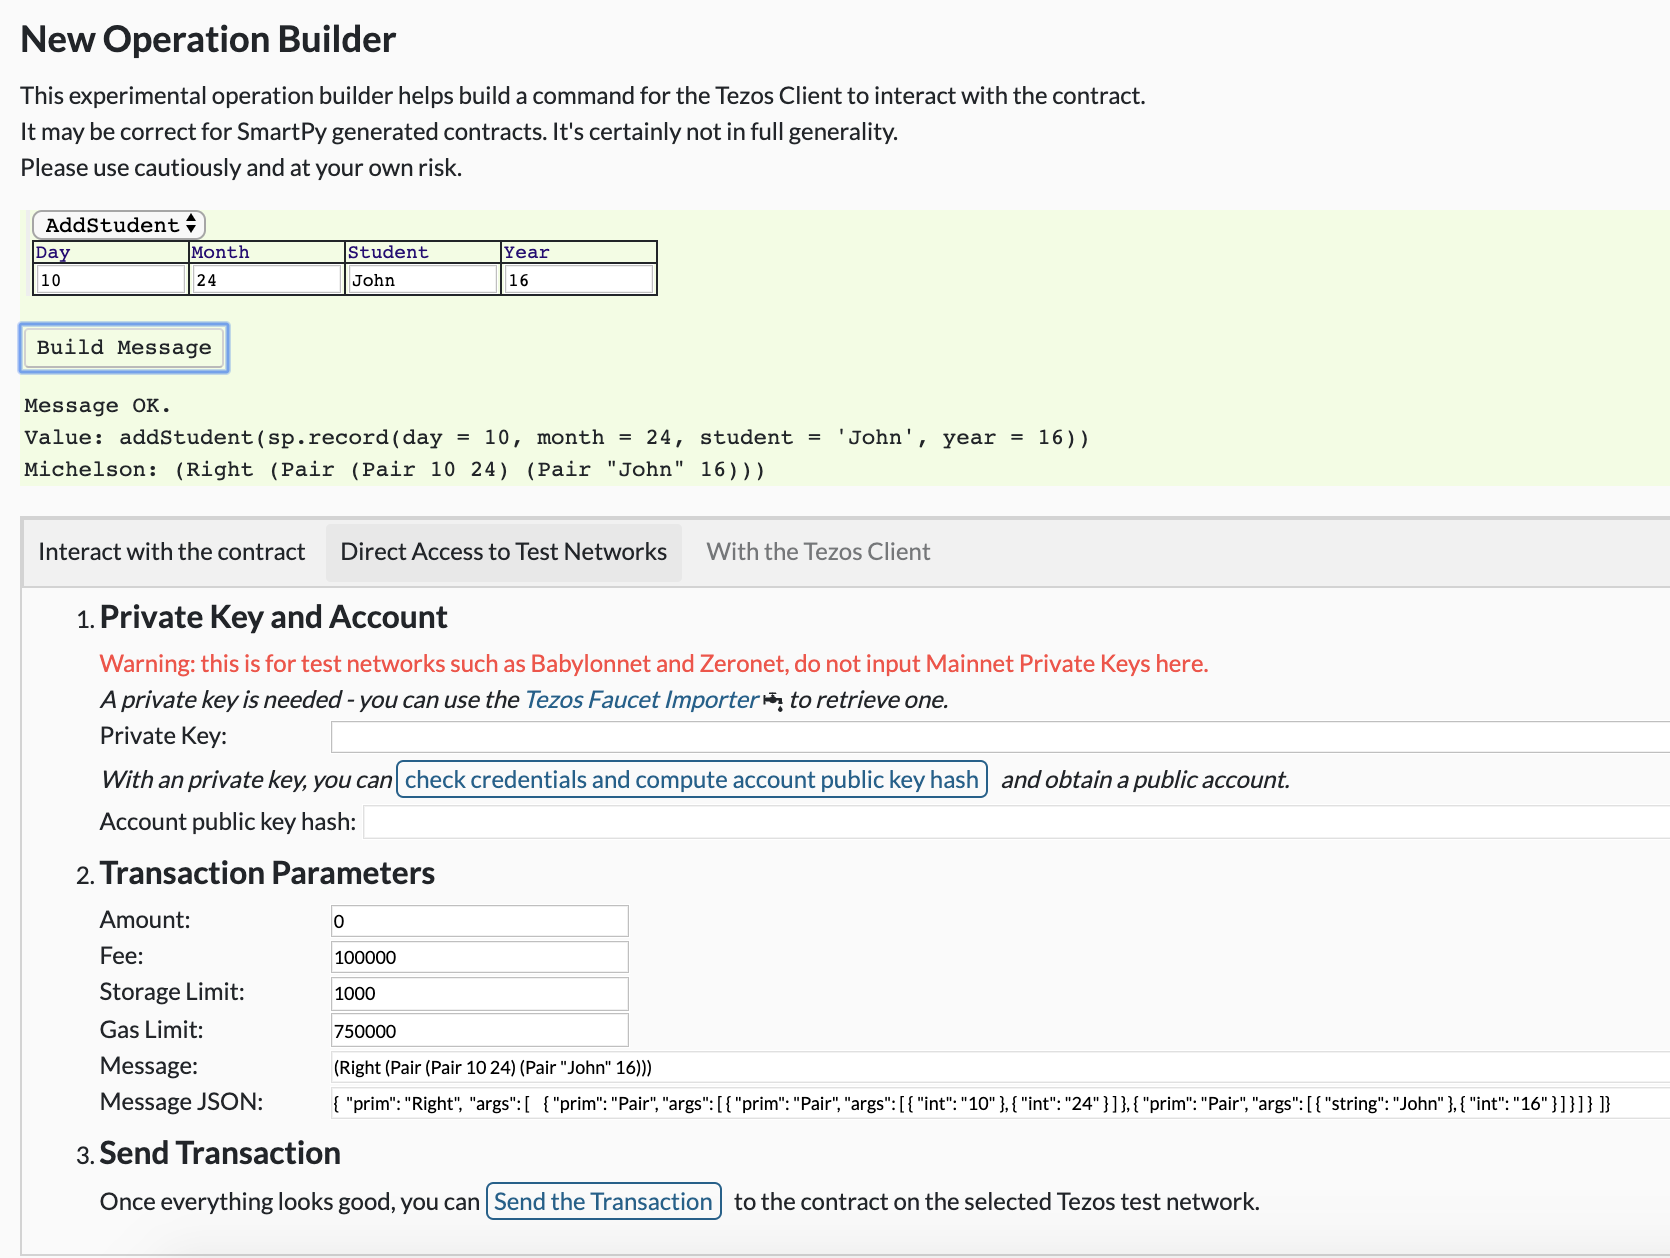
\includegraphics[scale=0.5]{operationbuilder}
\subsection{Testing Contract Transactions}
Each transaction is associated with a sender -- accessed using \lstinline!sp.sender! -- and a Tezos amount. The user should first select which entry point they would like to take using the "New Operation Builder" section, providing necessary parameters within the builder then selecting "Build Message." The user should then specify their private key (to identify them as a sender) and the transaction amount, finally selecting "Send the Transaction" to execute the desired transaction. The transaction will only succeed if the private key is valid and the smart contract deems that other necessary checks are in place. \\
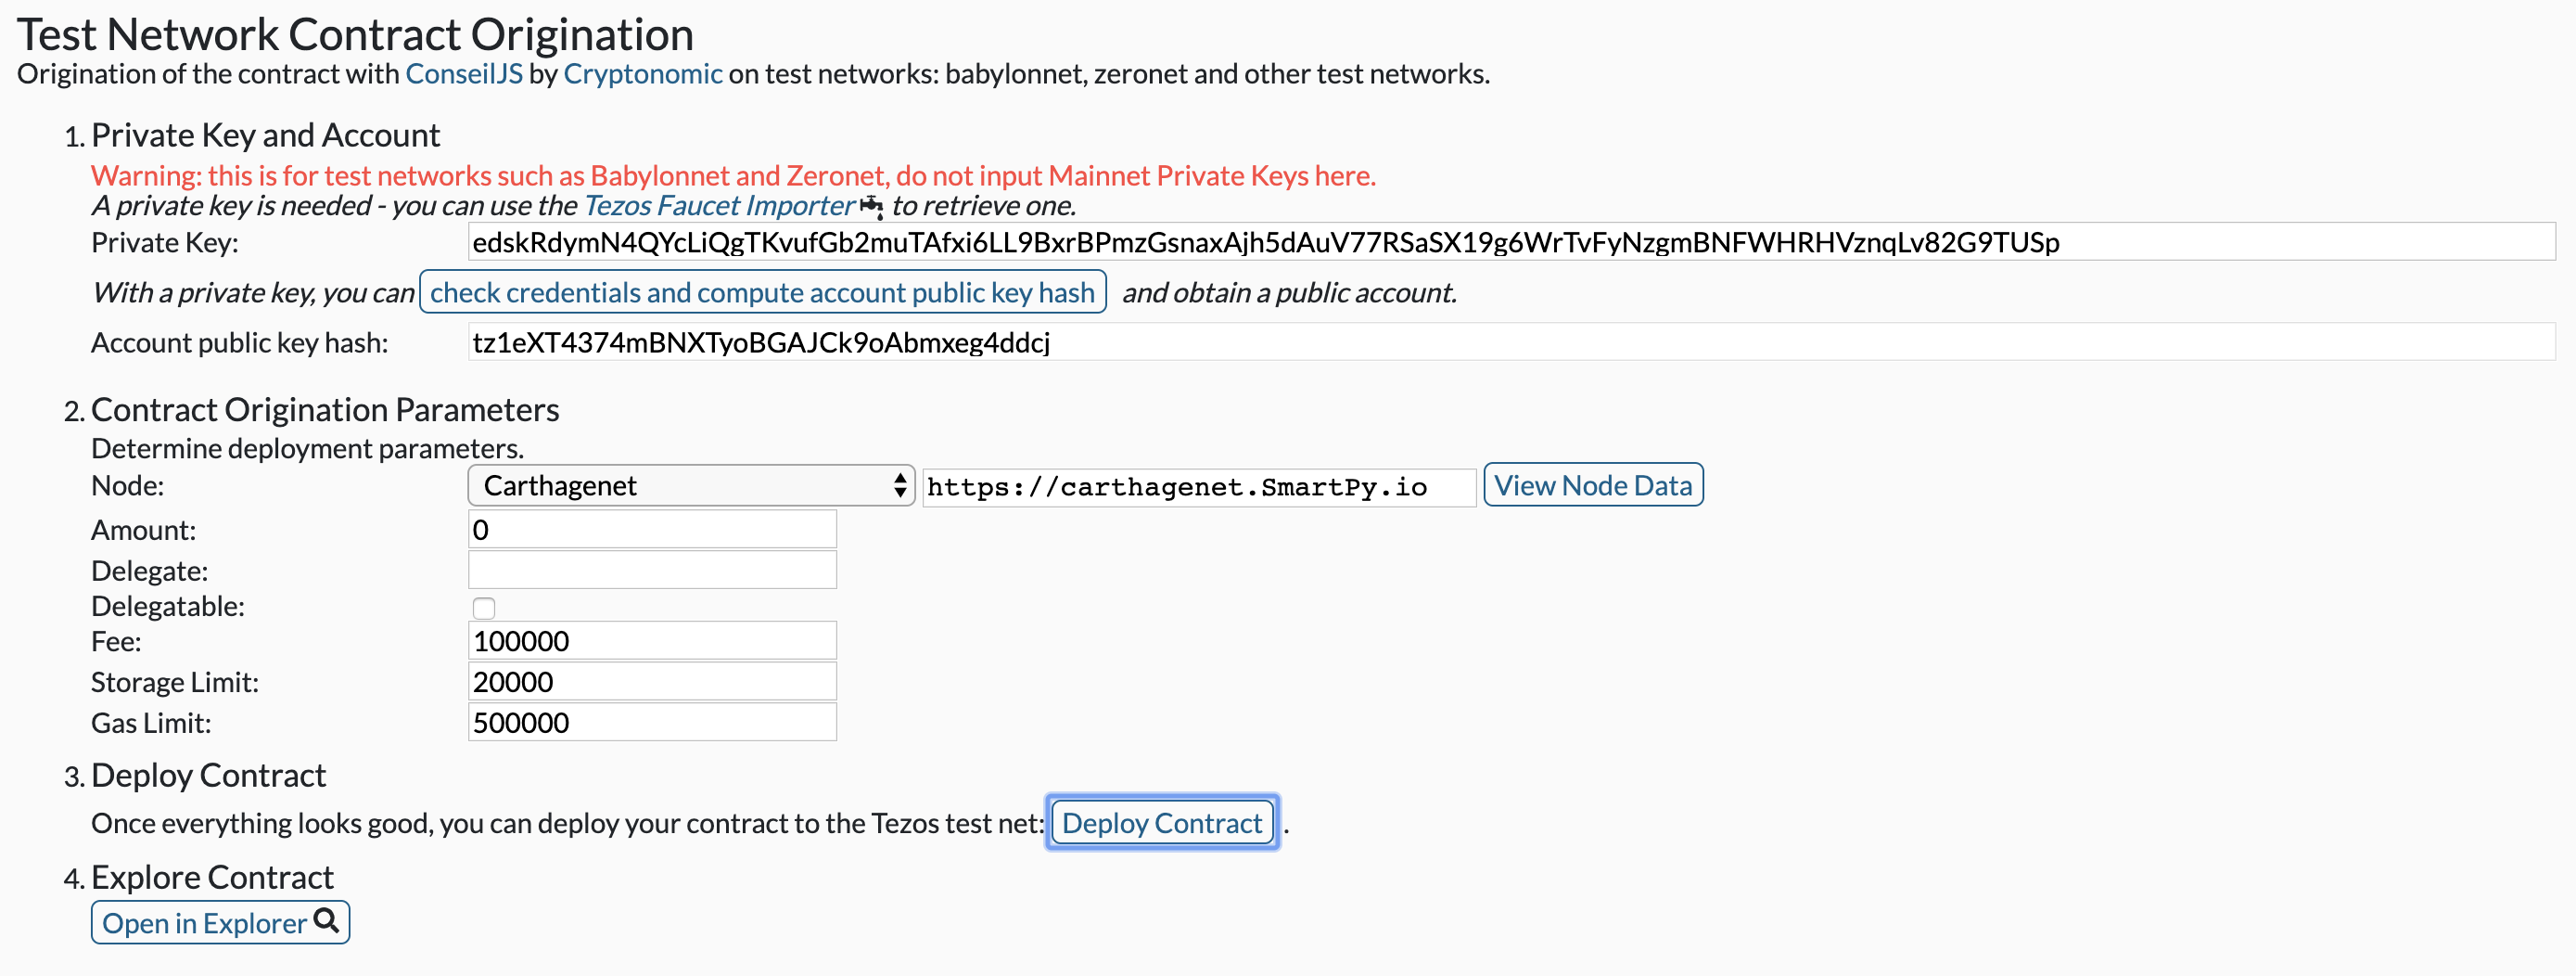
\includegraphics[scale=0.44]{origination}
\section{Conclusion}
This paper provides a summary of the syntactic subtleties of the SmartPy language and reports the steps necessary for deploying a smart contract to the testnet. However, yet to be explored is the element crucial to any successful smart contract, or the physical transfer of Tezos funds between two wallet addresses. SmartPy provides the support for this transaction in its Tezos-specific methods. Another necessary step will be deploying a developed and tested smart contract to the mainnet, which was not explored largely due to the Tezos fee associated with addings to the blockchain.
\end{document} 
